\documentclass[a4paper, amsfonts, amssymb, amsmath, reprint, showkeys, nofootinbib, twoside]{revtex4-1}
\usepackage[english]{babel}
\usepackage[utf8]{inputenc}
\usepackage[colorinlistoftodos, color=green!40, prependcaption]{todonotes}
\usepackage[pdftex, pdftitle={Article}, pdfauthor={Author}]{hyperref}
\usepackage{amsthm}
\usepackage{mathtools}
\usepackage{physics}
\usepackage{xcolor}
\usepackage{caption}
\usepackage{hyperref}
\usepackage{multirow}
\usepackage{amsmath}
\usepackage{amssymb}
\usepackage{graphicx}
\graphicspath{Images}
\usepackage[left=23mm,right=13mm,top=35mm,columnsep=15pt]{geometry} 
\usepackage{adjustbox}
\usepackage{placeins}
\usepackage[T1]{fontenc}
\usepackage{float}
%\usepackage{longtable}
\usepackage{csquotes}
\usepackage{refstyle}
\usepackage{lipsum}

\begin{document}

\title{Study of Mono-atomic and Di-atomic Lattice Vibrations With Electronic Circuits}
\author{Swaroop Ramakant Avarsekar}
\email{swaroop.avarsekar@niser.ac.in}
\affiliation{School of Physical Sciences, National Institute of Science Education and Research, HBNI, Jatni -752050, India}
\date{\today}
	
\begin{abstract}
	In this experiment we plan to construct analogy of mono atomic lattice and diatomic lattice with electronic circuits using capacitors and inductors building low pass LC filters. We study the dispersion relation for both these cases. We will calculate the cutoff frequency of the mono-atomic lattice, the frequency at the Brillouin zone boundary of both the optical and the acoustic branch of the diatomic lattice and estimate the energy of the bandgap in diatomic lattice. For monoatomic lattice we obtain cutoff frequency as (44.815$\pm$1.744) kHz. Frequency of optical mode Brillouin zone, $\nu_+$ (33.60$\pm$1.31) kHz. Frequency of acoustic mode Brillouin zone, $\nu_-$, (19.80$\pm$0.77) kHz. For Band gap energy, (57.072$\pm$3.14) peV. 
\end{abstract}
	
\keywords{Lattice constant, Acoustic Branch, Optical Branch, Lissajous figure.}
	
\maketitle

\section{Theory}
All solids have periodic arrays of atoms which form a crystal lattice except amorphous solids. Crystal lattice can be defined as the symmetrical 3d arrangement of atoms. Lattice vibrations is the displacement of the atoms/points from its equilibrium position. The crystal lattice vibrations can be replicated in a spring-mass model. Where the mass represents the atom and the spring represents the bonds or the lines connecting the points in a crystal lat- tice. With lattice constant being $a$, and array is infinitely long.

\begin{figure}[H]
	\centering
	\includegraphics[scale=0.25]{1} 
	\caption{1D monoatomic Lattice}
	\label{s}
\end{figure}

\begin{equation}
	m\ddot{x_n}=f((U_{n+1}+U_{n+1}) -2U_n)
\end{equation}

Solving above equation will give,
\begin{equation}
	\omega^2=2f(1-cos\theta)/m
\end{equation}

To get the frequency $\nu$,
\begin{equation}
	\nu=\omega/2\pi=\frac{\sqrt{2f(1-cos\theta)/m}}{2\pi}
\end{equation}

We get maximum frequency, by $\theta=0$. 
To measure the displacement of the mass in the spring mass model if high frequencies are used, with regular equipment. Thus a LC ladder circuit is used and a multi meter is used to measure the voltage and frequency of the signal.

\begin{figure}[H]
	\centering
	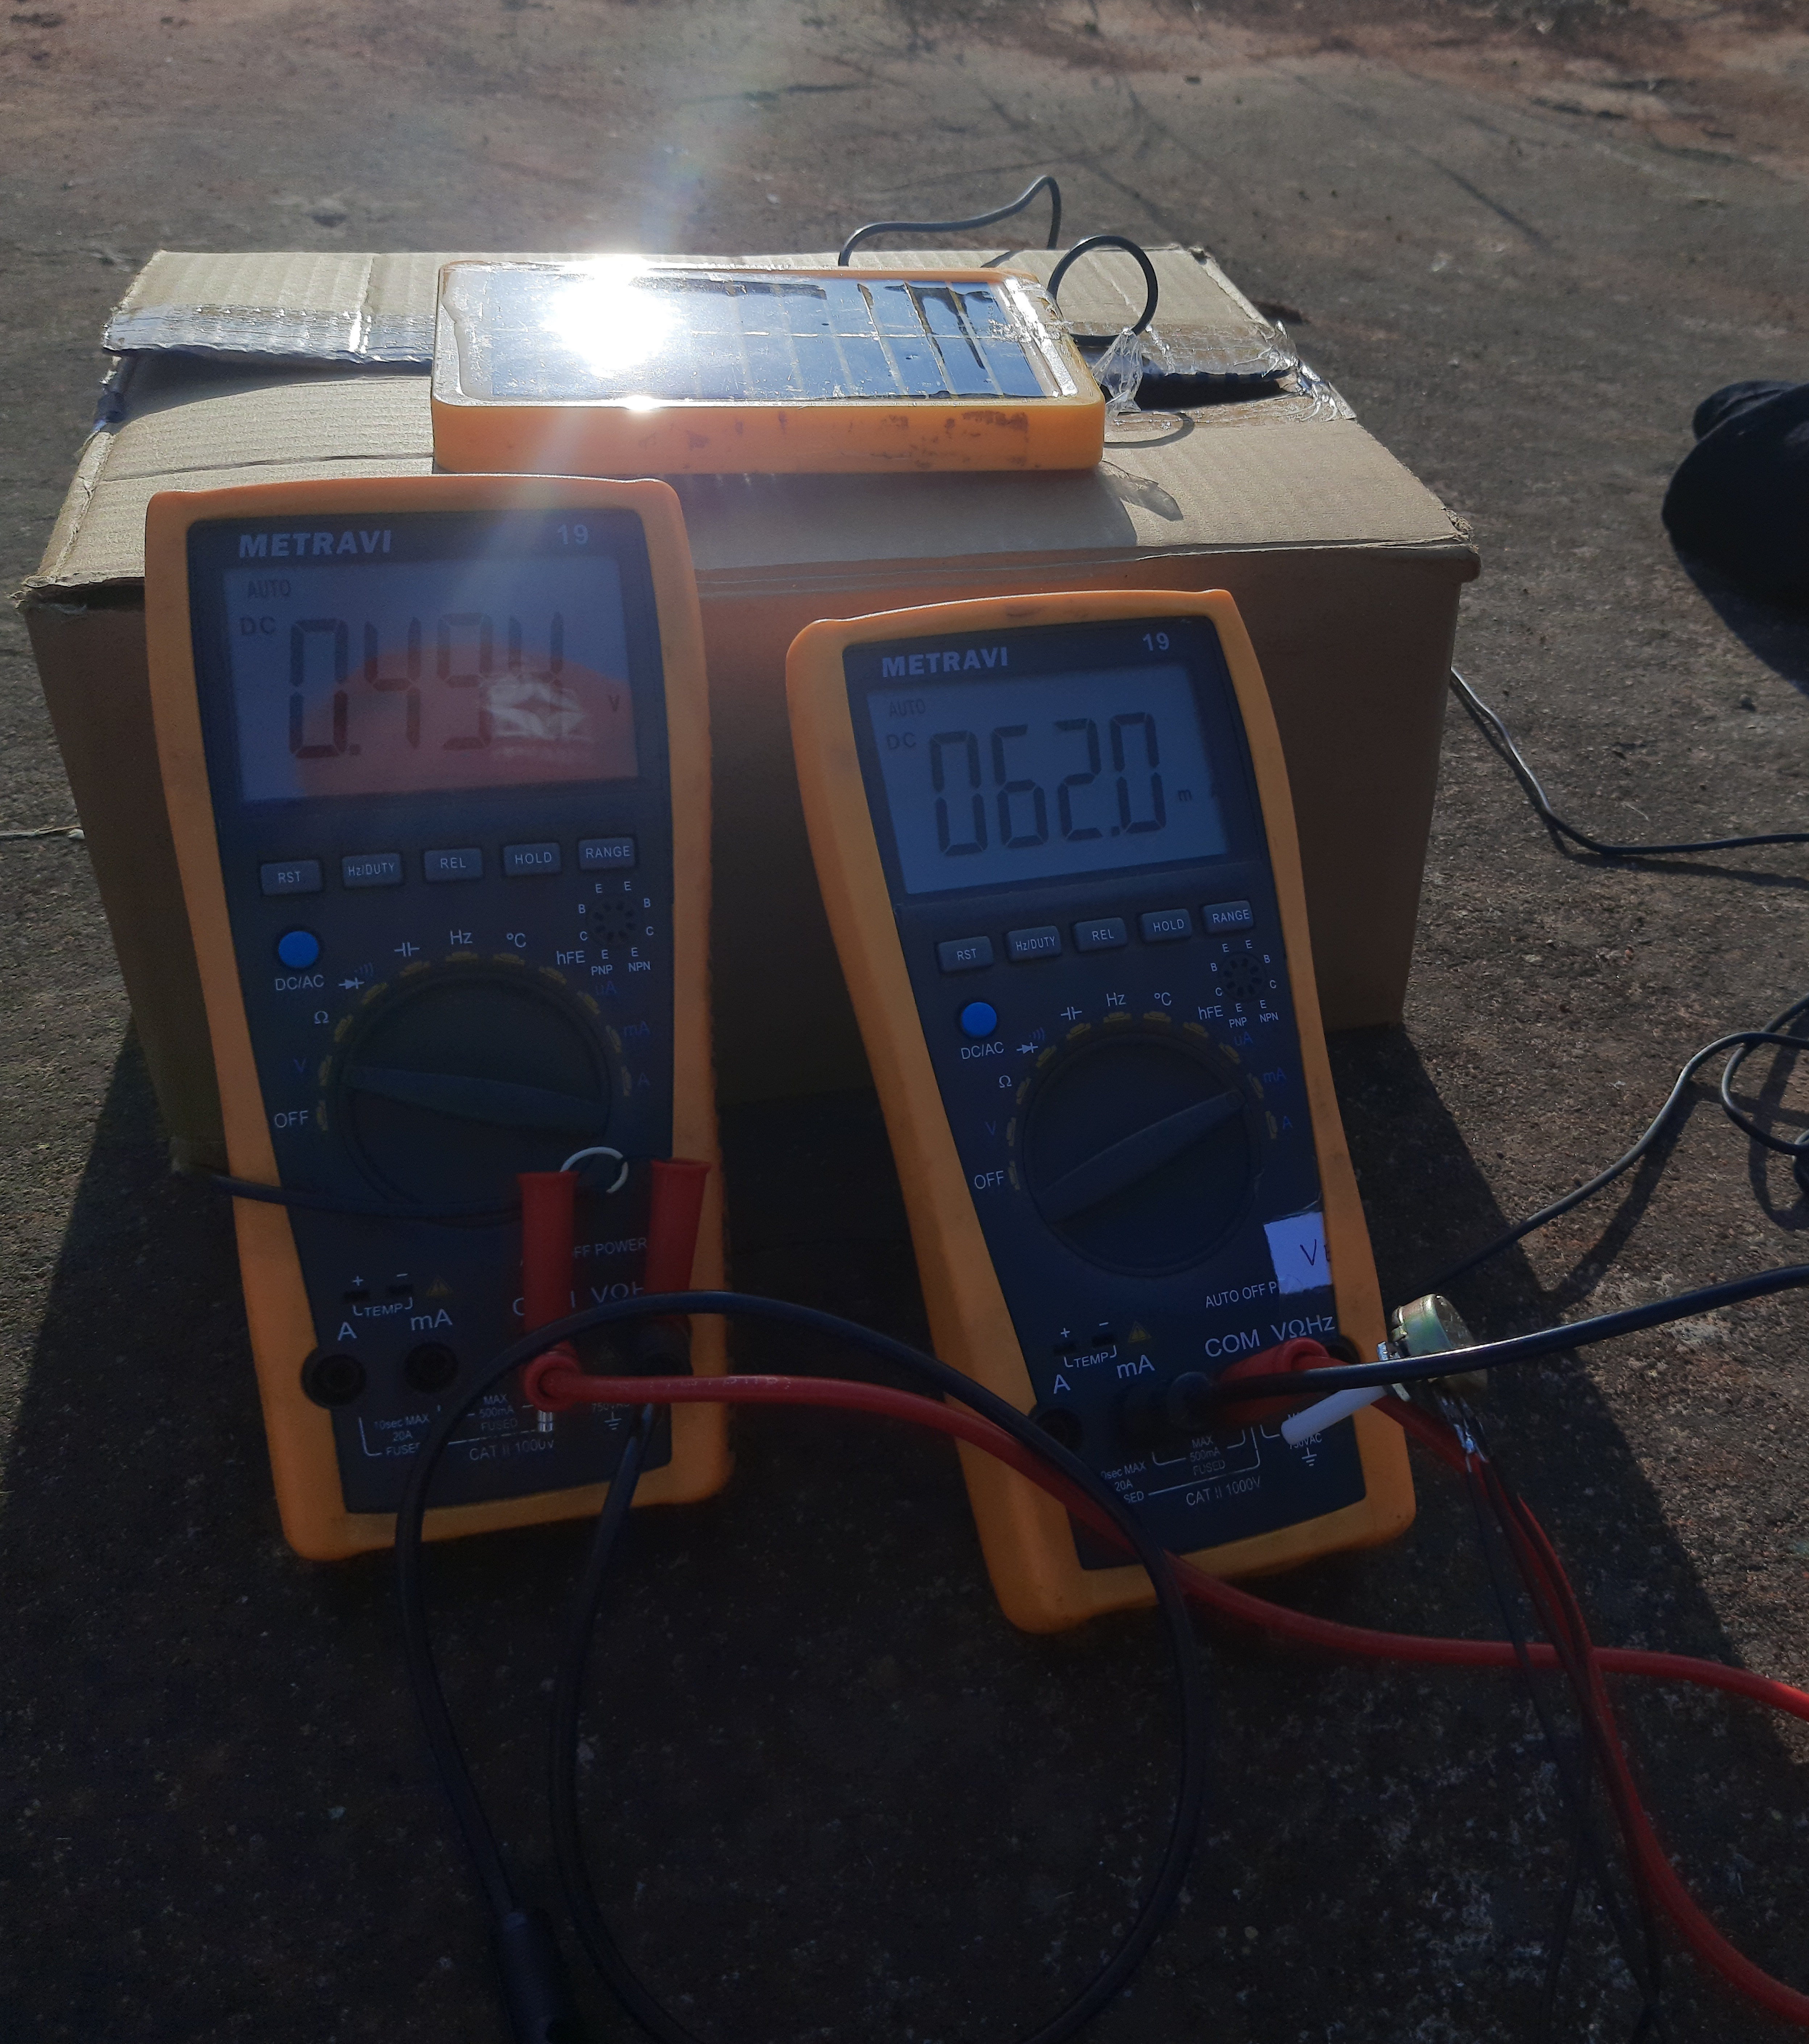
\includegraphics[scale=0.25]{2} 
	\caption{LC ladder}
	\label{s}
\end{figure}

For mono-atomic lattice equal no. of capacitors and inductors are used each with same values. Therefore the dispersion relation of circuit is 

\begin{equation}
	\omega^2=2(1-cos\theta)/LC
\end{equation}
where $\theta$ is the phase change. Thus, one
has a precise analogy with the one dimensional mono-atomic lattice with L being mass analog and 1/C being frequency analog. By measuring the phase difference between the input and output voltages of
the circuit shown in Fig. 2 as the function of frequency, the dispersion relation may be
verified.

\begin{figure}[H]
	\centering
	\includegraphics[scale=0.5]{3} 
	\caption{1D diatomic lattice}
	\label{s}
\end{figure}

\begin{figure}[H]
	\centering
	\includegraphics[scale=0.3]{4} 
	\caption{Electrical analog of diatomic lattice}
	\label{s}
\end{figure}

In diatomic lattice with alternative masses ‘M1’ and ‘M2’ shown in Fig.3 can be
simulated by the transmission line with alternative capacitors ‘C’ and ‘C1’ shown Fig.4. There are now two frequencies $\omega_+$ and $\omega_-$ for a particular wave vector k. leading two branches. The $\nu_-$ is acoustical branch and $\nu_+$ is optical branch. The frequency gap between the two branches depends on (M/m) $\leftrightarrow$ (C/C1)

\begin{figure}[H]
	\centering
	\includegraphics[scale=0.3]{5} 
	\caption{Dispersion relation for diatomic lattice}
	\label{s}
\end{figure}

\section{Experiment \& Analysis}
Monoatomic lattice was constructed using 10 inductors and capacitors. Diatomic with 10 capacitors with 5 similar capacitors each, while inductor being same. X-Y mode from oscilloscope displays lissajous figure.

\begin{figure}[H]
	\centering
	\includegraphics[scale=0.58]{m} 
	\caption{Frequency versus phase plot for monoatomic lattice}
	\label{s}
\end{figure}

\begin{table}[H]
	\centering
	\caption{Frequency and phase angle for monoatomic lattice}
	\label{t1}
		\begin{tabular}{|l|l|}
			\hline
			\begin{tabular}[c]{@{}l@{}}Frequency\\ (KHz)\end{tabular} & \begin{tabular}[c]{@{}l@{}}$\phi$ \\ (deg)\end{tabular} \\ \hline
			0.249  & 0    \\ \hline
			3.374  & 90   \\ \hline
			7.16   & 180  \\ \hline
			10.606 & 270  \\ \hline
			14.555 & 360  \\ \hline
			17.901 & 450  \\ \hline
			21.25  & 540  \\ \hline
			24.653 & 630  \\ \hline
			27.906 & 720  \\ \hline
			30.964 & 810  \\ \hline
			34     & 900  \\ \hline
			36.489 & 990  \\ \hline
			39.333 & 1080 \\ \hline
			41.586 & 1170 \\ \hline
			43.471 & 1260 \\ \hline
			44.815 & 1350 \\ \hline
		\end{tabular}
\end{table}

\begin{table}[H]
	\centering
	\caption{Frequency and phase angle for diatomic lattice}
	\label{t2}
		\begin{tabular}{|l|l|}
			\hline
			$\phi$ & \begin{tabular}[c]{@{}l@{}}Frequency \\ (kHz)\end{tabular} \\ \hline
			90     & 2.4                                                        \\ \hline
			180    & 5.1                                                        \\ \hline
			270    & 7.6                                                        \\ \hline
			360    & 10.2                                                       \\ \hline
			450    & 12.4                                                       \\ \hline
			540    & 14.7                                                       \\ \hline
			630    & 16.6                                                       \\ \hline
			720    & 18.3                                                       \\ \hline
			810    & 19.8                                                       \\ \hline
			900    & 33.6                                                       \\ \hline
			990    & 35                                                         \\ \hline
			1080   & 36.2                                                       \\ \hline
			1170   & 37.4                                                       \\ \hline
		\end{tabular}
\end{table}

\begin{figure}[H]
	\centering
	\includegraphics[scale=0.58]{d} 
	\caption{Frequency versus phase plot for diatomic lattice}
	\label{s}
\end{figure}

\begin{table}[H]
	\centering
	\caption{Capacitance and Inductance values}
	\label{t2}
		\begin{tabular}{|l|ll|}
			\hline
			L(mH) & \multicolumn{1}{l|}{C1(nF)}        & C2(nF)       \\ \hline
			1.082 & \multicolumn{1}{l|}{254}           & 819          \\ \hline
			0.993 & \multicolumn{1}{l|}{avg=50.8 nF}   & avg=163.8 nF \\ \hline
			0.992 & \multicolumn{2}{l|}{\multirow{7}{*}{}}            \\ \cline{1-1}
			0.978 & \multicolumn{2}{l|}{}                             \\ \cline{1-1}
			1.058 & \multicolumn{2}{l|}{}                             \\ \cline{1-1}
			1.033 & \multicolumn{2}{l|}{}                             \\ \cline{1-1}
			1.039 & \multicolumn{2}{l|}{}                             \\ \cline{1-1}
			1.043 & \multicolumn{2}{l|}{}                             \\ \cline{1-1}
			1.081 & \multicolumn{2}{l|}{}                             \\ \hline
			0.976 & \multicolumn{1}{l|}{avg=1.0275 mH} &              \\ \hline
		\end{tabular}
\end{table}

Value of inductance for harmonic and alternating chain is $(1.028\pm0.040)$ mH. Capacitance for harmonic chain is 51.3 nF, where 10 capacitors were used. Capacitance for alternating chain is 50.8 nF and 163.8 nF, where 5 capacitors each were used.

From experiment, for monoatomic lattice we obtain cutoff frequency as 44.815 kHz. Frequency of optical mode Brillouin zone, $\nu_+$ 33.6 kHz. Frequency of acoustic mode Brillouin zone, $\nu_-$, 19.8 kHz.

Band gap energy E,
\begin{equation}
	E=h(\nu_+-\nu_-)
\end{equation}

\begin{equation}
	E=h(33.6-19.8)\times10^{3}=57.072 ~peV
\end{equation}

To calculate theoretical cutoff frequency for monoatomic lattice, we have
\begin{equation}
	\nu=\frac{1}{\pi}\sqrt{\frac{1}{LC}}
\end{equation}

For diatomic lattice,
\begin{equation}
	\nu_{\pm}=\frac{1}{\pi}\sqrt{\frac{2}{LC_{1/2}}}
\end{equation}

From these equations, we obtain theoretical cutoff frequency for monoatomic lattice as 43.38 kHz and for diatomic lattice, optical mode frequency as 31.146 kHz and acoustic mode frequency as 17.345 kHz.

Theoretical band gap energy,
\begin{equation}
	E=h(31.146-17.345)\times10^3=57.076~ peV
\end{equation}

Relative error in cutoff frequency of harmonic chain,
\begin{equation}
	\frac{44.815-43.38}{43.38}.100\%=3.3\%
\end{equation}

Relative error in optical frequency,
\begin{equation}
	\frac{33.6-31.146}{31.146}.100\%=7.8\%
\end{equation}

Relative error in acoustic frequency,
\begin{equation}
	\frac{19.8-17.345}{17.345}.100\%=14.15\%
\end{equation}

Relative error in band gap energy,
\begin{equation}
	\frac{57.076-57.072}{57.076}.100\%=0.007\%
\end{equation}

Propagation of error ,

For cutoff frequency of harmonic chain,
\begin{equation}
	\delta \nu=\nu.\sqrt{\left( \frac{\delta L}{L}\right) ^2+\left( \frac{\delta C}{C}\right) ^2}=1.744 kHz
\end{equation}

For optical frequency,
\begin{equation}
	\delta \nu_+=\nu_+.\sqrt{\left( \frac{\delta L}{L}\right) ^2+\left( \frac{\delta C_1}{C_1}\right) ^2}=1.308 kHz
\end{equation}

For acoustical frequency,
\begin{equation}
	\delta \nu_-=\nu_-.\sqrt{\left( \frac{\delta L}{L}\right) ^2+\left( \frac{\delta C_2}{C_2}\right) ^2}=0.77 kHz
\end{equation}

For band gap energy
\begin{equation}
	\delta E=E.\sqrt{\left( \frac{\delta \nu_-}{\nu_-}\right) ^2+\left( \frac{\delta \nu_+}{\nu_+}\right) ^2}=3.14 peV
\end{equation}

Therefore, for monoatomic lattice we obtain cutoff frequency as (44.815$\pm$1.744) kHz. Frequency of optical mode Brillouin zone, $\nu_+$ (33.60$\pm$1.31) kHz. Frequency of acoustic mode Brillouin zone, $\nu_-$, (19.80$\pm$0.77) kHz. For Band gap energy, (57.072$\pm$3.14) peV. 

The relative error for each of these parameters are 3.3\%, 7.8\%, 14.15\% and 0.007\%, respectively.

\section{Conclusion}
From this experiment we successfully constructed the electrical circuit using inductors and capacitors as the analogue of monoatomic and diatomic lattice vibration. For monoatomic lattice we obtain cutoff frequency as (44.815$\pm$1.744) kHz. Frequency of optical mode Brillouin zone, $\nu_+$ (33.60$\pm$1.31) kHz. Frequency of acoustic mode Brillouin zone, $\nu_-$, (19.80$\pm$0.77) kHz. For Band gap energy, (57.072$\pm$3.14) peV. 

The relative error for each of these parameters are 3.3\%, 7.8\%, 14.15\% and 0.007\%, respectively. The error was tried to be reduced by increasing no. of unit cells, but this contributed to noise. Other errors contributing to this experiment are the fluctuating phase angle due to frequency generators or determining phase angles through lissajous figures, usually at higher frequencies the output is not accurate. The value of  inductors and capacitors used was not equal, hence periodic unit is not identical. 

\section{References}
\begin{enumerate}
\item{SPS NISER Lab Manual}
\item{\url{https://unlcms.unl.edu/cas/physics/tsymbal/teaching/SSP-927/Section%2005_Lattice_Vibrations.pdf}}
%\item {\url{}}
%\item {\url{}}
\end{enumerate}

\end{document}